\newpage
\chapter{Chapter}
\section{Section}
\subsection{Subsection}
\subsubsection{Subsubsection}
My text here with \textbf{italics}, with \textbf{bold}, and a \href{https://davibarreira.github.io/}{link}.  Adding some math expression here with $x=10$ and $y = 10^2 + 2*2$. $x=10$Adding some math expression here with $x=10$ and $y = 10^2 + 2*2$. $y = 10^2 + 2*2$Adding some math expression here with $x=10$ and $y = 10^2 + 2*2$. 
\begin{displaymath}
	d(\omega(t_0),\omega(t_1)) \leq \int^{t_1}_{t_0}g(s) ds.
\end{displaymath} Adding some code like  \lstinline{plots}. Note that the  \lstinline{using plots} """ 
\begin{lstlisting}[language=JuliaLocal, style=julia]
using PlutoUI
\end{lstlisting}

\begin{lstlisting}[language=JuliaLocal, style=julia]
begin
	using Plots
	y(x) = sin(x)
	plot(y,
		color=:blue)
end
\end{lstlisting}

\begin{figure}[H]
	\centering
	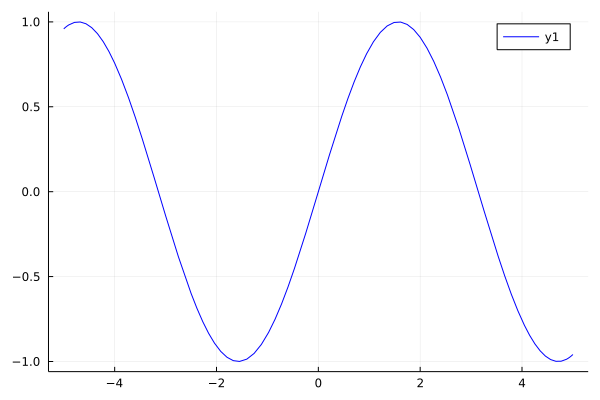
\includegraphics[width=0.8\textwidth]{./figures/examplepluto_figure1.png}
	\label{fig:examplepluto_figure1.png}

\end{figure}

\begin{lstlisting}[language=JuliaLocal, style=julia]
A = [10,10,10]
\end{lstlisting}

\begin{verbatim}
3-element Vector{Int64}:
 10
 10
 10
\end{verbatim}

\begin{lstlisting}[language=JuliaLocal, style=julia]
x = rand(10);
\end{lstlisting}

\begin{lstlisting}[language=JuliaLocal, style=julia]
x .+ 1
\end{lstlisting}

\begin{verbatim}
10-element Vector{Float64}:
 1.9889812668868116
 1.3810127256277165
 1.2397163891072562
 1.8032076294063573
 1.7136510187553888
 1.029653815677927
 1.661858529215337
 1.5725020169642838
 1.0552107425727795
 1.13156902006914
\end{verbatim}

\begin{lstlisting}[language=JuliaLocal, style=julia]
set_theme!(theme_ggplot2())
\end{lstlisting}

\begin{lstlisting}[language=JuliaLocal, style=julia]
Makie.plot(x)
\end{lstlisting}

\begin{figure}[H]
	\centering
	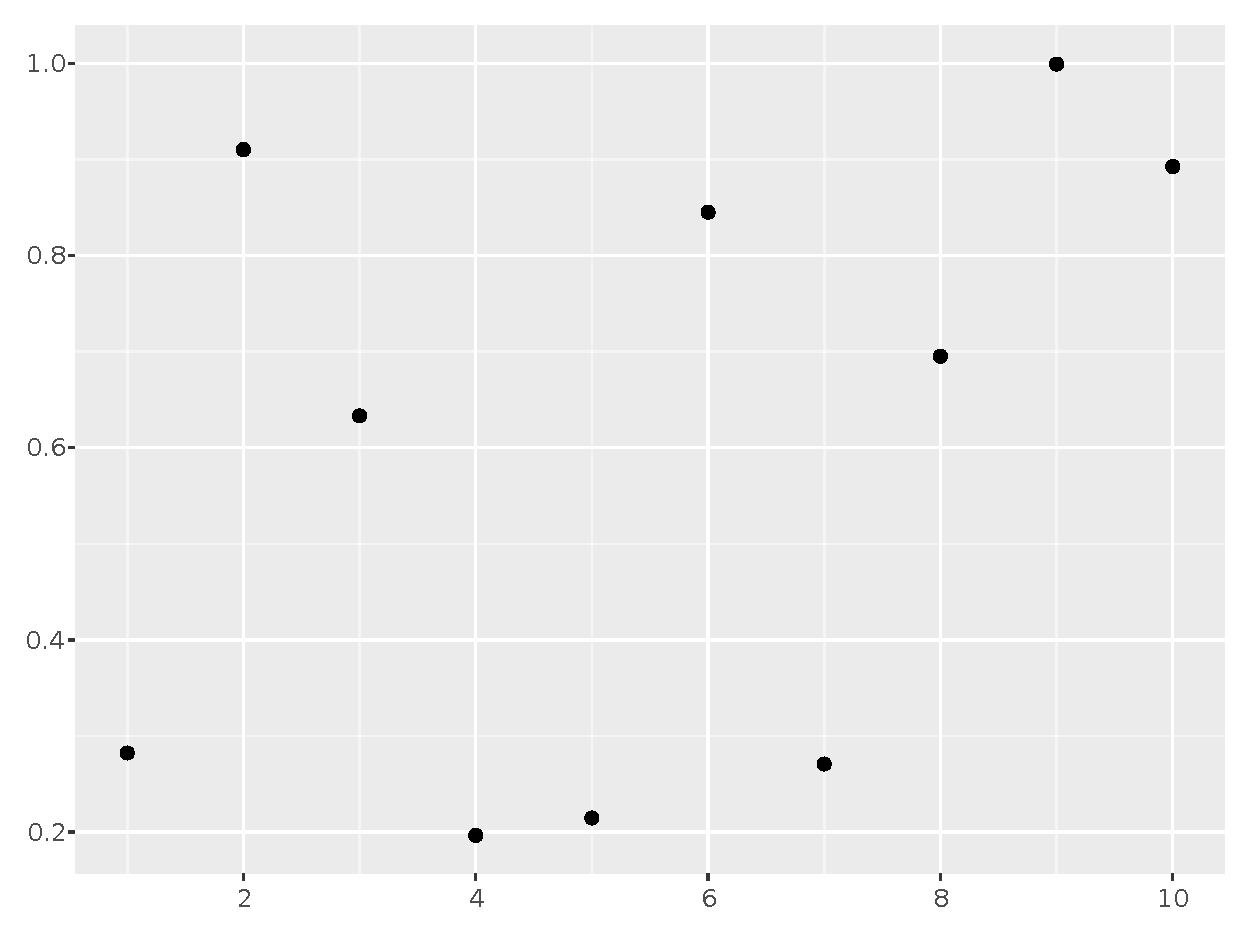
\includegraphics[width=0.8\textwidth]{./figures/examplepluto_figure2.pdf}
	\label{fig:examplepluto_figure2.pdf}

\end{figure}

\begin{lstlisting}[language=JuliaLocal, style=julia]
PlutoUI.LocalResource(figurepath)
\end{lstlisting}

\begin{figure}[H]
	\centering
	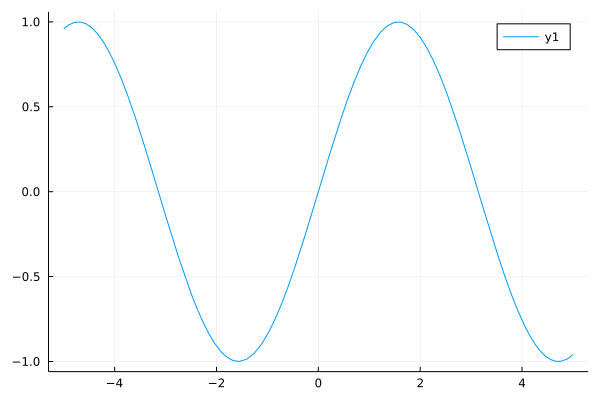
\includegraphics[width=0.8\textwidth]{/home/davibarreira/MEGA/EMAp/NotebookToLatex.jl/example/plotexample.png}
	\label{fig:/home/davibarreira/MEGA/EMAp/NotebookToLatex.jl/example/plotexample.png}

\end{figure}
